\documentclass[12pt, letterpaper, notitlepage, twoside]{article}
\usepackage[letterpaper,bindingoffset=0in,%
            left=1in,right=1in,top=1in,bottom=1in,%
            footskip=.25in]{geometry}
\usepackage{mathtools}
\usepackage{graphicx}
\usepackage{setspace}
\usepackage{amsmath}
\usepackage{amsfonts}
\usepackage{amsthm}
\usepackage{amssymb}
\usepackage{csquotes}
\usepackage{relsize}
\usepackage{tikz}
\usetikzlibrary{cd}
\usepackage{hhline}
\usepackage{systeme}
\usepackage{mathrsfs}
\usepackage{hyperref}
\usepackage{mathtools}  

\theoremstyle{definition}
\newtheorem{df}{Definition}
\newtheorem{exa}{Example}
\newtheorem{exr}{Exercise}
\newtheorem*{note}{Note}
\theoremstyle{plain}
\newtheorem{thm}{Theorem}
\newtheorem{prop}{Proposition}
\newtheorem{conj}{Conjecture}
\newtheorem{cor}{Corollary}
\newtheorem{lm}{Lemma}
\usepackage[ruled]{algorithm2e}

\usepackage{ulem}
\makeatletter

\def\lf{\left\lfloor}   
\def\rf{\right\rfloor}
\def\st{\text{ s.t. }}
\def\1{^{-1}}
\def\nrmll{\trianglelefteq}
\def\nrmlr{\trianglerighteq}
\def\R{\mathbb{R}}
\def\Q{\mathbb{Q}}
\def\Z{\mathbb{Z}}
\def\C{\mathbb{C}}
\def\I{\mathbb{I}}
\newcommand{\leg}[2]{\left( \frac{#1}{#2} \right)}
\renewcommand*\env@matrix[1][*\c@MaxMatrixCols c]{%
   \hskip -\arraycolsep
   \let\@ifnextchar\new@ifnextchar
   \array{#1}}
\makeatother
\renewcommand{\mod}[1]{\ (\mathrm{mod}\ #1)}
\let\oldsqrt\sqrt
\def\sqrt{\mathpalette\DHLhksqrt}
\def\DHLhksqrt#1#2{%
\setbox0=\hbox{$#1\oldsqrt{#2\,}$}\dimen0=\ht0
\advance\dimen0-0.2\ht0
\setbox2=\hbox{\vrule height\ht0 depth -\dimen0}%
{\box0\lower0.4pt\box2}}
\usepackage{float}
\restylefloat{figure}

\usepackage{cleveref}
\Crefname{thm}{Theorem}{Theorems}

\begin{document}
Kyle Dituro \hfill \today

James McClung
\begin{center}
{\huge Assignment 3}
\end{center}

\section{Training Results}
\begin{center}
    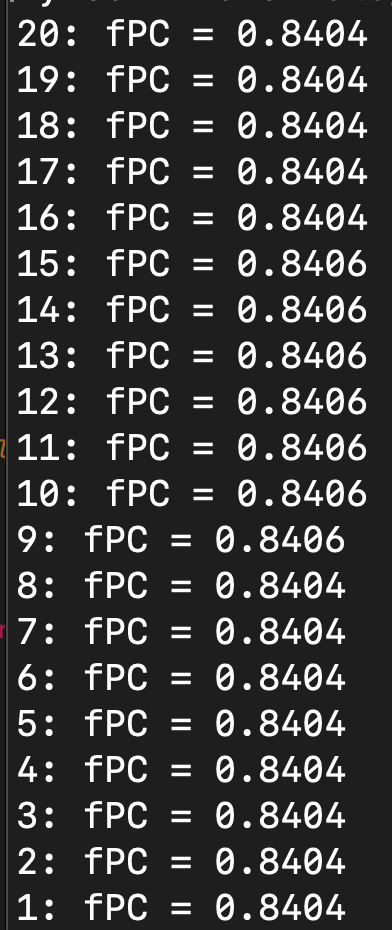
\includegraphics{Imgs/fPC.png}
    
    \textbf{fPC of last 20 epochs}

    \pagebreak
    
\includegraphics{Imgs/results.png}

    \textbf{Training results}
\end{center}

\section{Weight Visualization:}
\begin{center}
    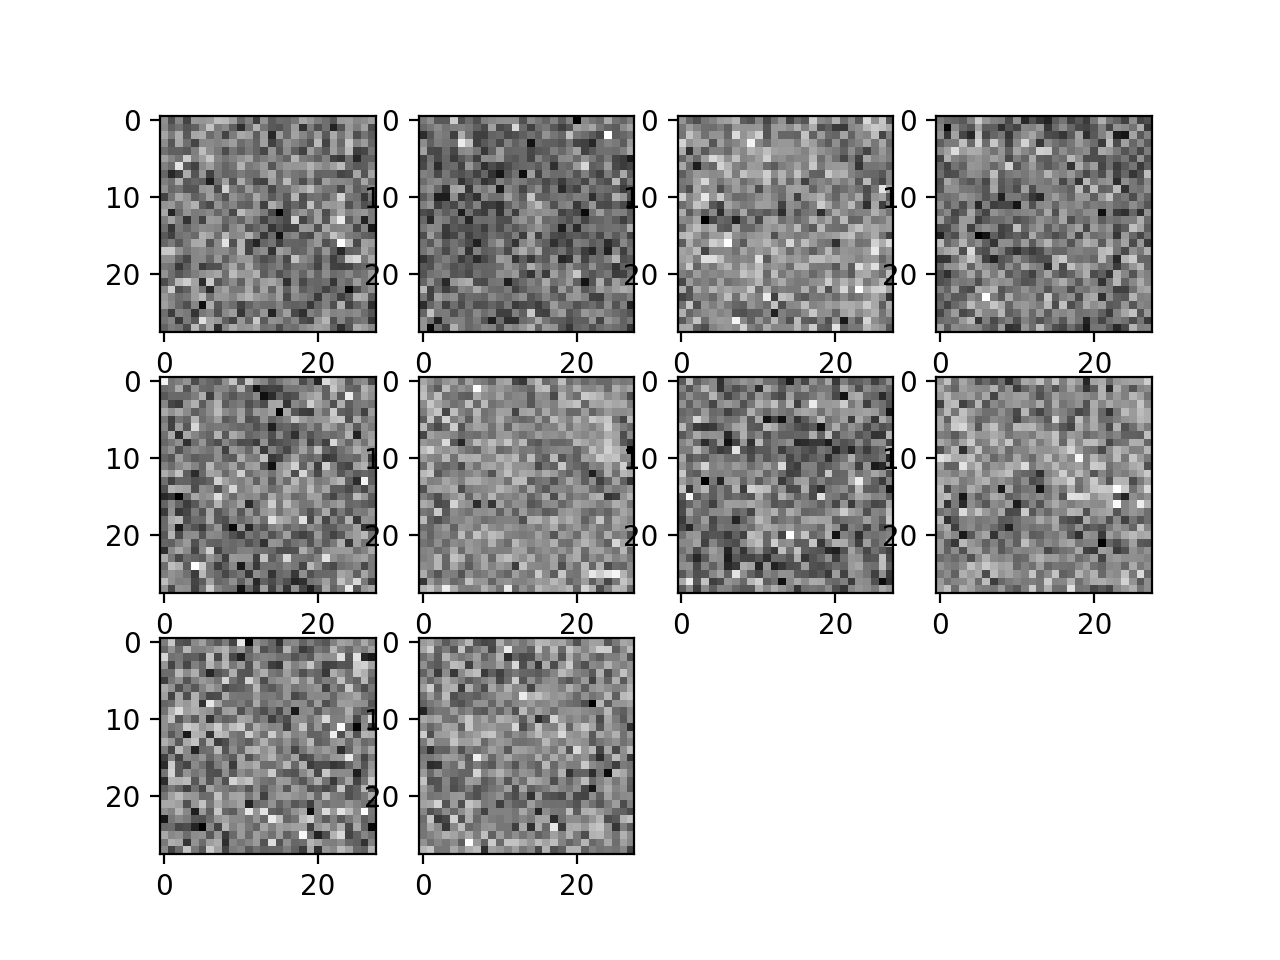
\includegraphics{Imgs/Wgray.png}
    \textbf{The charts above correspond to weights according to the below table}
    \begin{tabular}{| c | c | c | c |}
    \hline
        0 & 1 & 2 & 3 \\
    \hline
        4 & 5 & 6 & 7 \\
    \hline
        8 & 9 & & \\
    \hline
    \end{tabular}
\end{center}

\section{Transformations:}
\begin{center}
    


    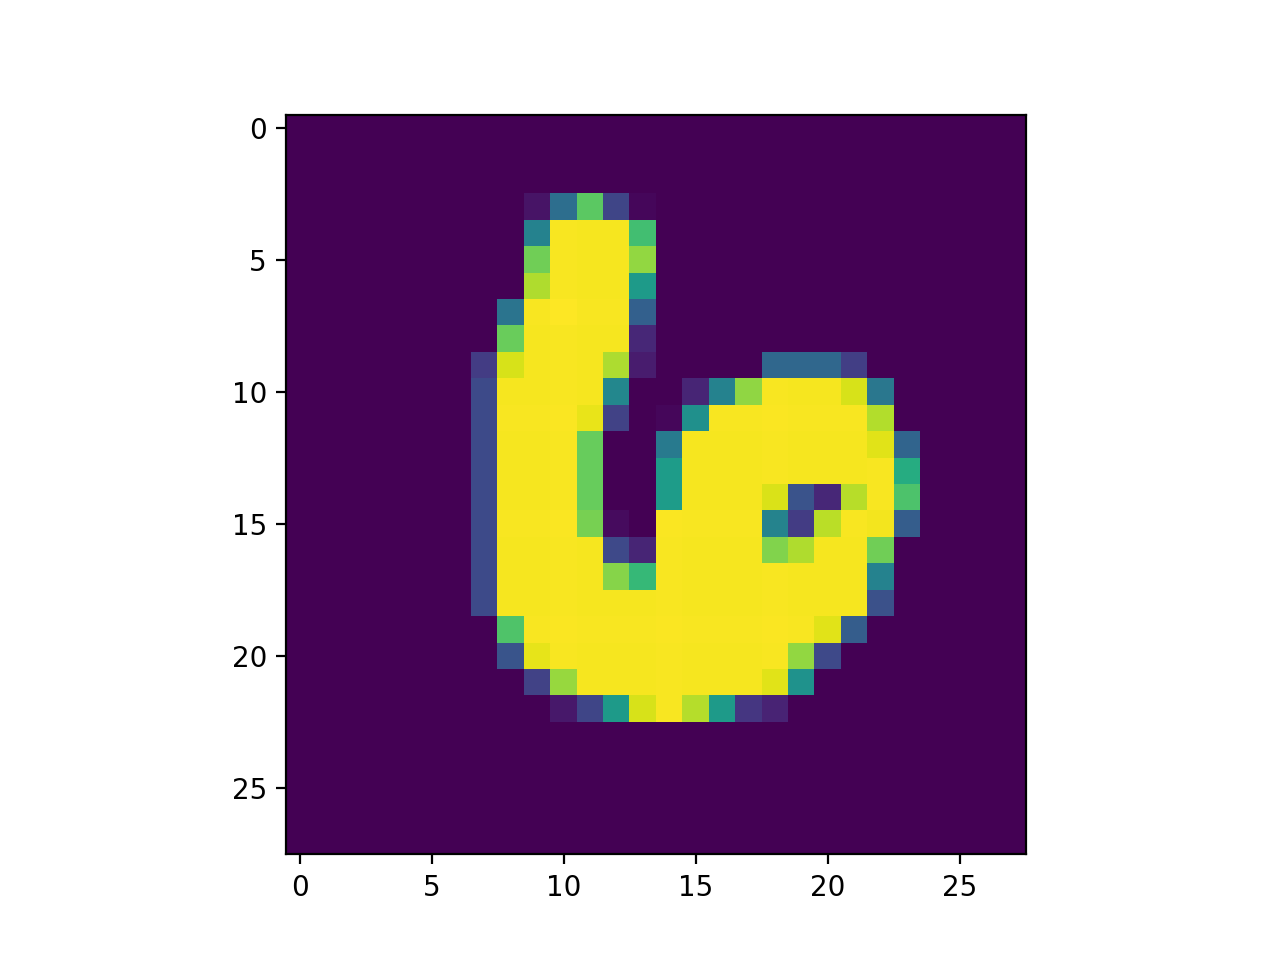
\includegraphics{Imgs/6.png}
    \textbf{Regular Image}

    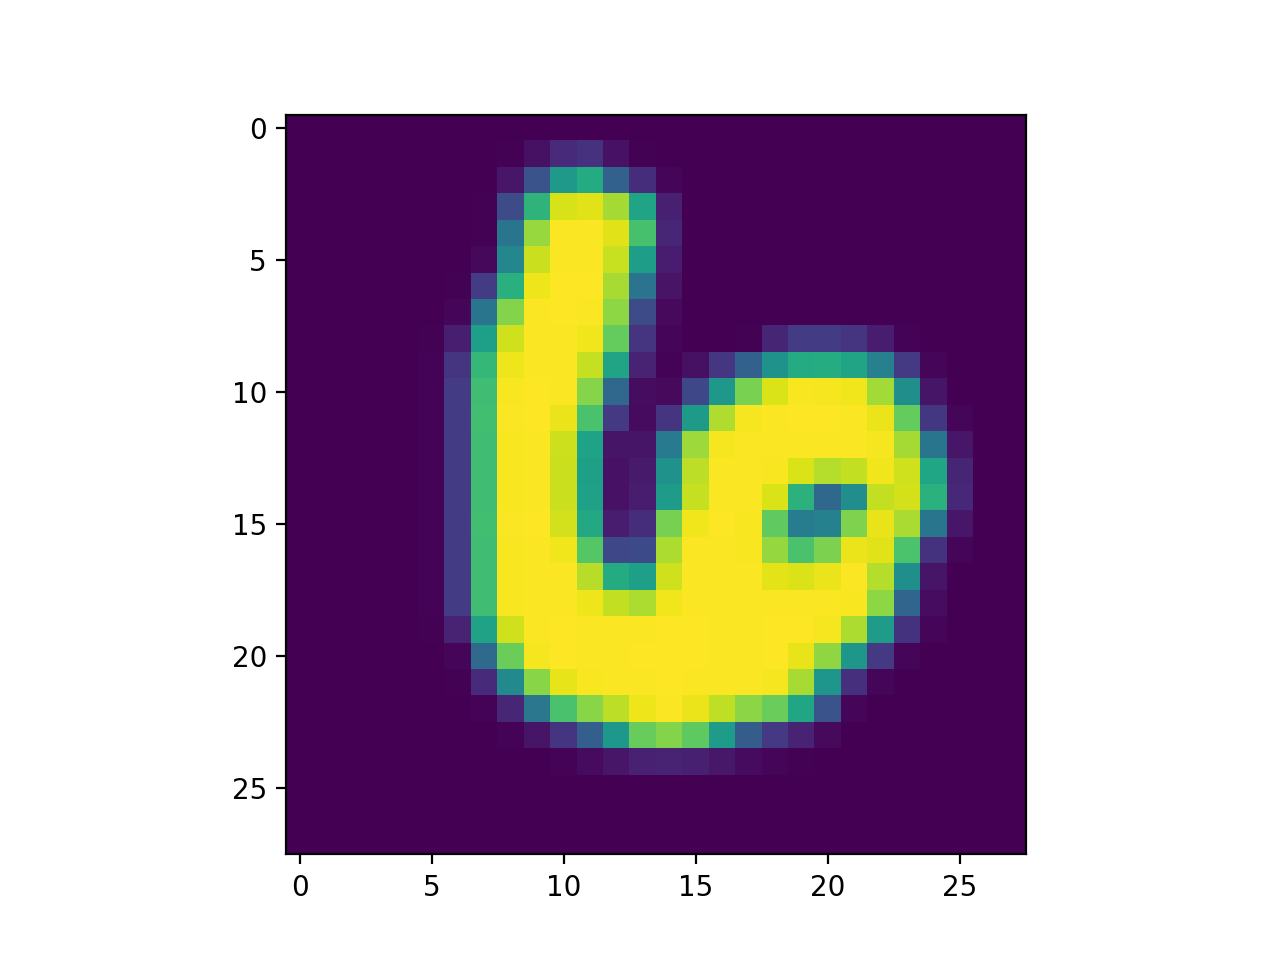
\includegraphics{Imgs/6_big.png}
    \textbf{Scaled Image}

    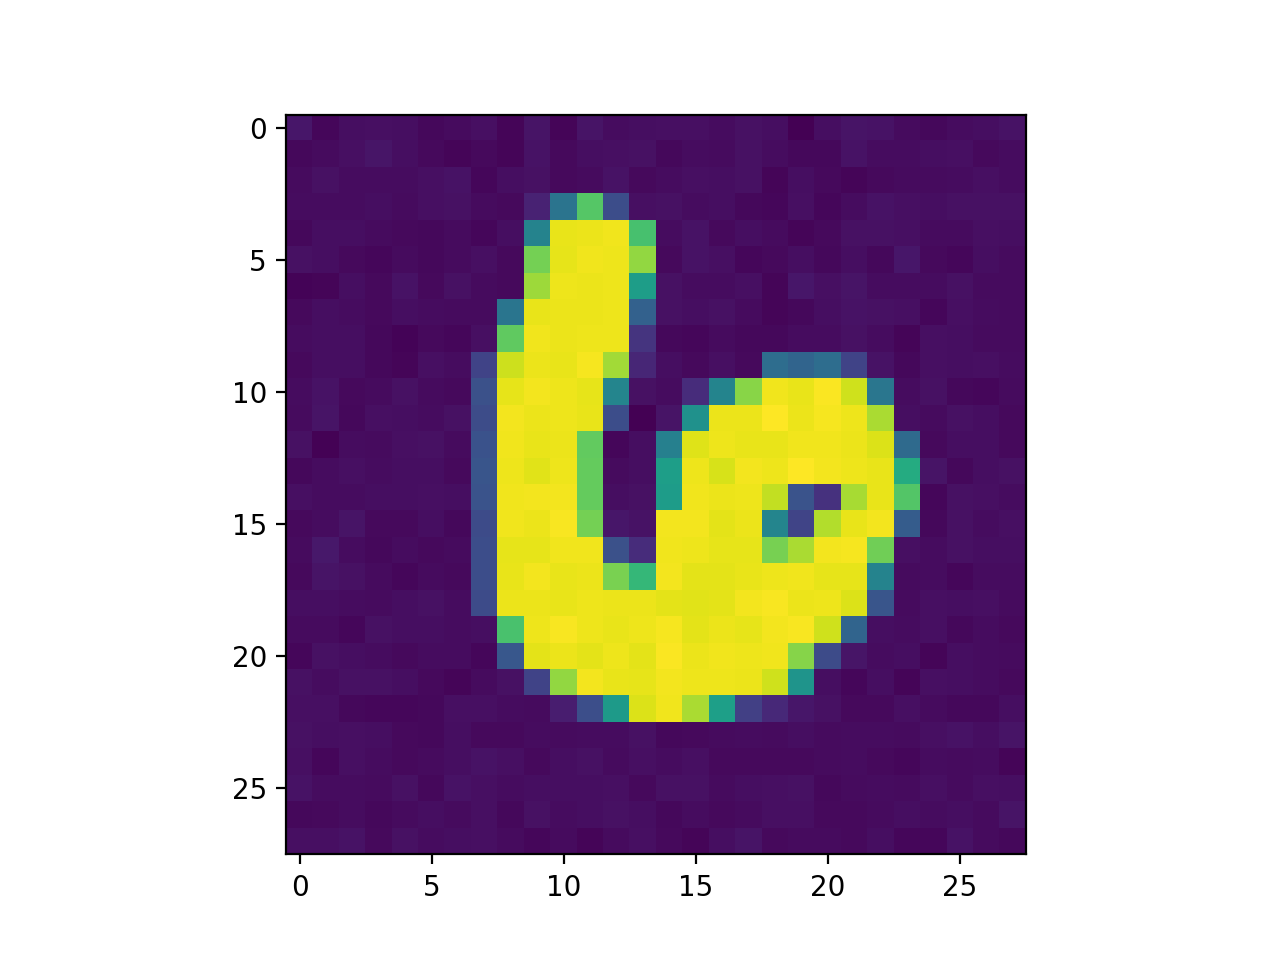
\includegraphics{Imgs/6_noise.png}
    \textbf{Noise Applied}

    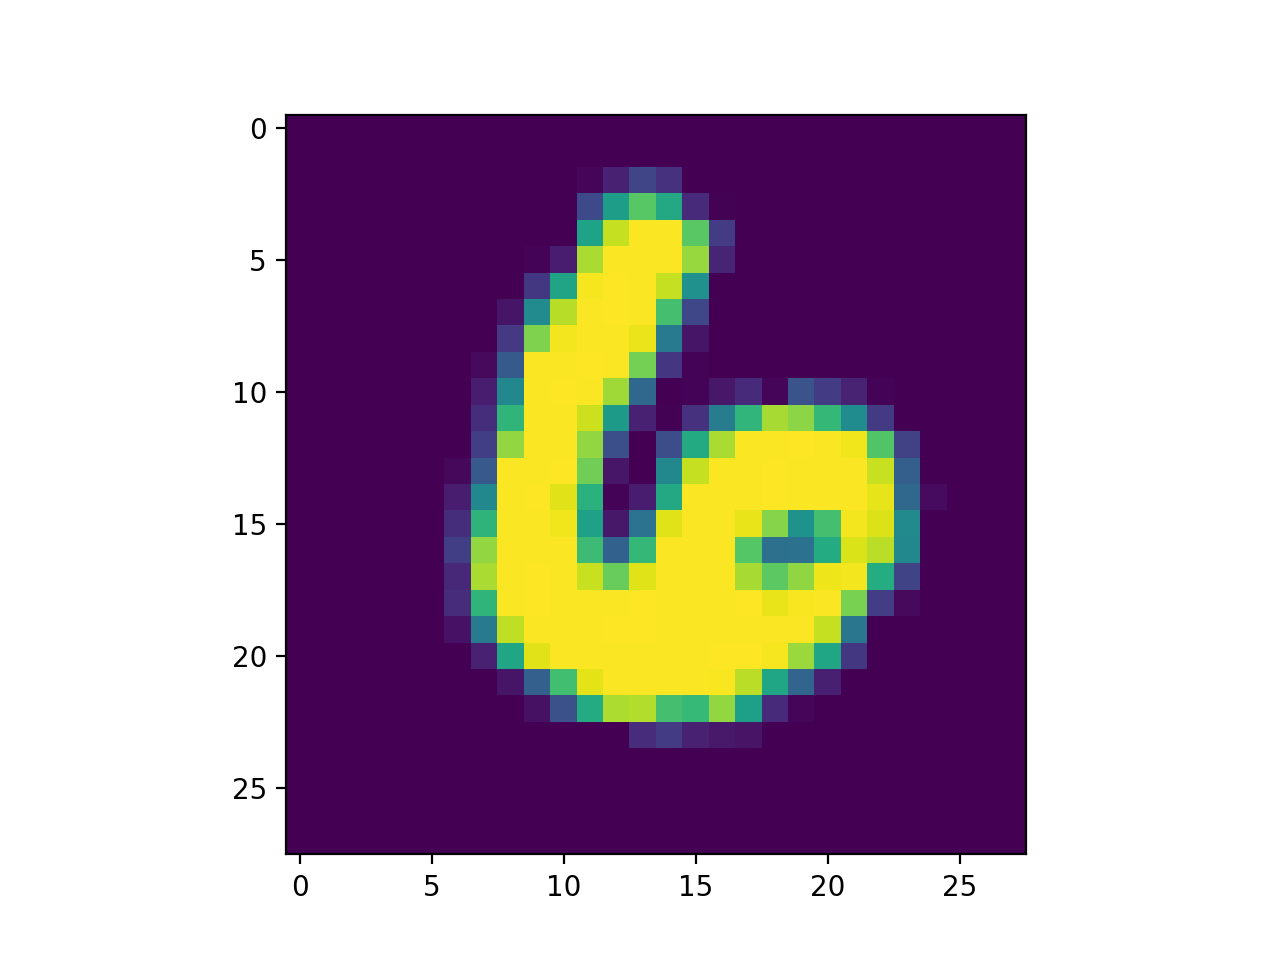
\includegraphics{Imgs/6_rot.png}
    \textbf{Rotated Image}

    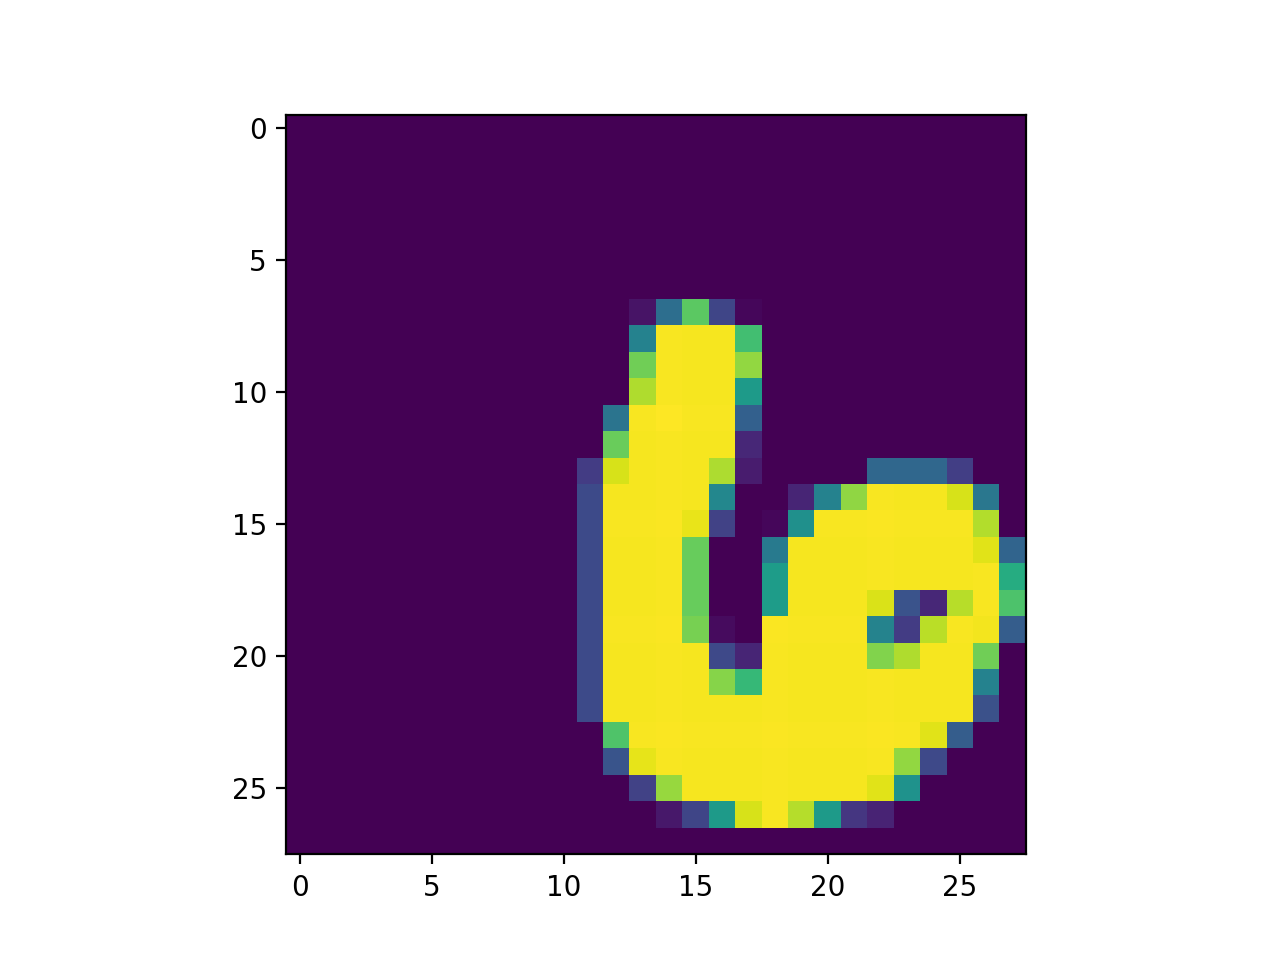
\includegraphics{Imgs/6_trans.png}
    \textbf{Translated Image}
\end{center}
\end{document}